\documentclass[12pt,letterpaper]{article}
\usepackage[utf8]{inputenc}
\usepackage[francais]{babel}
\usepackage[T1]{fontenc}
\usepackage{amsmath}
\usepackage{amsfonts}
\usepackage{amssymb}
\usepackage{graphicx}

\newcommand{\mb}[1]{\mathbf{#1}}
\newcommand{\norm}[1]{\left\lVert#1\right\rVert}

\author{Jordan Longval}
\title{Cable crossing developement}
\begin{document}
\maketitle
To help with the development, it helps to look at figure 1. 
\begin{figure}[!h]
\centering
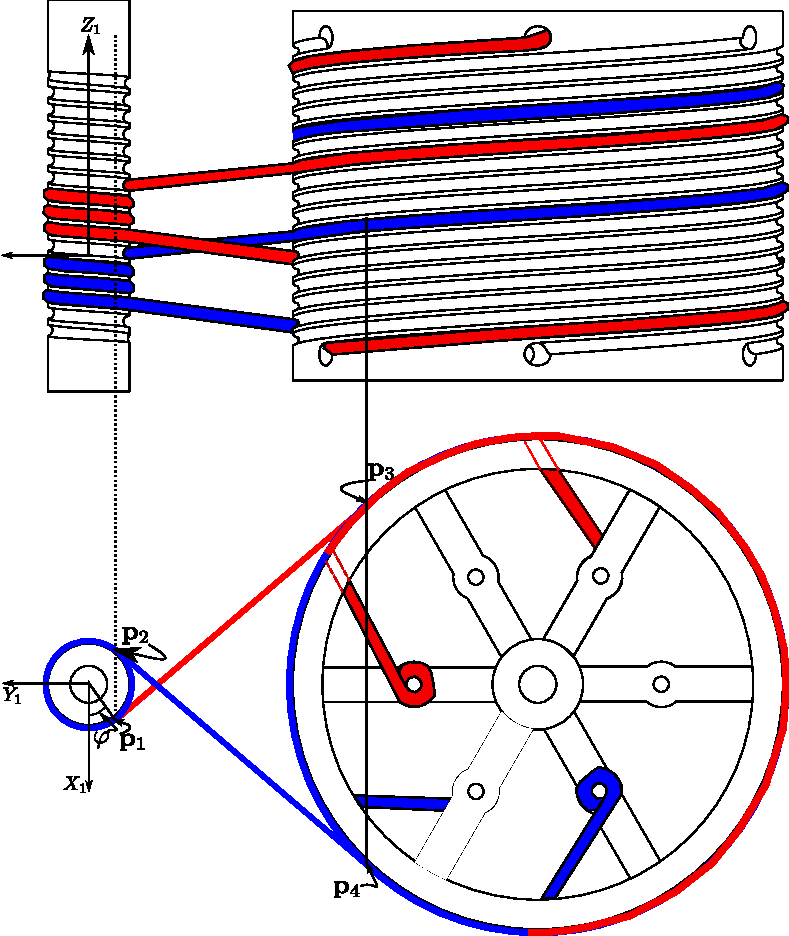
\includegraphics[width=0.6\textwidth]{fig_1.pdf} 
\caption{cable crossing condition.}
\end{figure}
The values of $\mathbf{p}_1$ and $\mathbf{p}_2$ are given by
\begin{align}
\mathbf{p}_1 = \begin{bmatrix}
r_1c\varphi\\
-r_1s\varphi\\\frac{H_1\varphi}{2\pi}
\end{bmatrix},\quad \mathbf{p}_2 = \begin{bmatrix}
-r_1c\varphi\\-r_1s\varphi\\\frac{H_1}{2\pi}(3\pi-\varphi).
\end{bmatrix}
\label{eq_1}
\end{align}
Also, we know that at points $\mathbf{p}_1$ and $\mathbf{p}_2$ the unit vectors that are tangeant and that go in the same direction as the cables (towards the large pulley) are expressed respectively as
\begin{align}
\mathbf{u}_1 = \frac{\begin{bmatrix}
-r_1s\varphi\\
-r_1c\varphi\\
\frac{H_1}{2\pi}
\end{bmatrix}}{\rho_1},
\quad \mathbf{u}_2 = \frac{\begin{bmatrix}
r_1s(3\pi-\varphi)\\
r_1c(3\pi-\varphi)\\
\frac{-H_1}{2\pi}
\end{bmatrix}}{\rho_1}=\frac{\begin{bmatrix}
r_1s\varphi\\
-r_1c\varphi\\
\frac{-H_1}{2\pi}
\end{bmatrix}}{\rho_1}.
\label{eq_2}
\end{align}
With the expressions in \eqref{eq_1} and \eqref{eq_2}, we can express the positions of $\mathbf{p}_3$ and $\mathbf{p}_4$ respectively as 
\begin{align}
\mathbf{p}_3 = \mathbf{p}_1 + L_f\mathbf{u}_1,\\ \mathbf{p}_4 = \mathbf{p}_2 + L_f\mathbf{u}_2.
\end{align}
The line $l_1$ that passes through $\mathbf{p}_1$ and $\mathbf{p}_2$ can be expressed with the form
\begin{align}
l_1: \mathbf{p}(s_1) = \mathbf{p}_1 + (\mathbf{p}_3-\mb{p}_1)s_1, \quad s_1 \in \mathbb{R},\label{eq_5}
\end{align}
where $s_1$ is an arbitrary parameter.
In the same manner, the line $l_2$ that passes through points $\mb{p}_3$ and $\mb{p}_4$ can be expressed with the form \begin{align}
l_2: \mathbf{p}(s_2) = \mathbf{p}_2 + (\mathbf{p}_4-\mb{p}_2)s_2, \quad s_2 \in \mathbb{R},\label{eq_6}
\end{align}
where $s_2$ is also an arbitrary parameter. The expressions in equations \eqref{eq_5} and \eqref{eq_6} can be further simplified to 
\begin{align}
l_1: \mb{p}(s_1) = \mb{p}_1 + L_fs_1\mb{u}_1, \quad l_2:\mb{p}(s_2) = \mb{p}_2 + L_fs_2\mb{u}_2.
\end{align}
The shortest distance $d$ between $l_1$ and $l_2$ is given by the following equation
\begin{align}
d =L_f^2\frac{\mb{u}_1\times\mb{u}_2}{\norm{\mb{u}_1\times\mb{u}_2}}\cdot\left(\mb{p}_2-\mb{p}_1\right). \\
L_f^2 = \frac{\rho^2_1\left(D^2-(r_2+r_1)^2\right)}{r_1^2}\\
\mb{u}_1\times\mb{u}_2 = \frac{1}{\rho_1^2}\begin{bmatrix}
-r_1s\varphi\\
-r_1c\varphi\\
\frac{H_1}{2\pi}
\end{bmatrix}\times
\begin{bmatrix}
r_1s\varphi\\
-r_1c\varphi\\
\frac{-H_1}{2\pi}
\end{bmatrix} = \frac{2r_1c\varphi}{\rho_1^2}\begin{bmatrix}
\frac{H_1}{2\pi}\\0\\r_1s\varphi
\end{bmatrix}\\
\norm{\mb{u}_1\times\mb{u}_2} = 
\end{align}
\end{document}